\documentclass[a4paper]{report}
\usepackage[]{amsmath}
\usepackage[]{physics} % \bra, \ket etc
\usepackage{graphicx} %Pour les figures je crois
\usepackage{hyperref}
\usepackage[
    backend=biber, 
    natbib=true,
    style=numeric,
    sorting=none, %Pour faire apparaitre les refs dans l'ordre
    hyperref=true
]{biblatex} %Imports biblatex package
\addbibresource{Bib_ch2.bib} %Import the bibliography file

\usepackage{subcaption} % package pour faire des subfigures
\usepackage{multirow} % package pour multirow/multicolumn
\usepackage{booktabs} % package pour top/mid/bottom rule
\usepackage{tcolorbox} % toujours plus de boites
\usepackage{xcolor} % Pour avoir des couleurs dans les équations

\title{Appendix A : Dipole-dipole interaction between two spins in solid}
\begin{document}
\chapter{Detection of dark spins via cross-relaxations}
In this chapter, we will see how...
\section{Flip-Flops, double flips and cross-relaxation}

\begin{figure}
\centering
\includegraphics[width=0.9\textwidth]{Figures/Shema_CR}
\caption{Illustration of cross-relaxations between an NV center and an unpolarized spin. Red dots represent the population in each states, and the arrows the various population transfer mechanisms}
\label{CR_shema}
\end{figure}

The dominant form of interaction between two distant spins is the magnetic dipole-dipole interaction. For two spins with with vector spin Hamiltonian $\hat{\mathbf{S}}_1$ and $\hat{\mathbf{S}}_2$, separated by a distance $\mathbf{r}=r\mathbf{u}$, the dipole-dipole interaction Hamiltonian reads (see Appendix A) :
\begin{equation}
\mathcal{H}_{dd}=\frac{J_0}{r^3}\left[ \hat{\mathbf{S}}_1\cdot\hat{\mathbf{S}}_2 - 3 (\hat{\mathbf{S}}_1\cdot\mathbf{u})(\hat{\mathbf{S}}_2\cdot\mathbf{u})\right],
\end{equation}
where $J_0= \frac{\mu_0\gamma_1\gamma_2 \hbar^2}{4\pi}$. For two electronic spins with $g-$factors close to 2 (which is the case for the NV center and most spin defect in diamond), the numerical value of $J_0$ is $(2\pi)\,52\ \rm{MHz}\cdot\rm{nm}^3$.

Flip-flop, in the context of dipole-dipole interaction, is the mechanism which exchanges a quantum of spin between two spins. For an initial state of two spins $\ket{m_s^1=i;m_s^2=j}$, a flip-flop process will result in a final state $\ket{i+1;j-1}$ or $\ket{i-1;j+1}$. The effective rate of this process depends on the matrix element $\mel{i;j}{\mathcal{H}_{dd}}{i\pm 1;j \mp 1}$, as well as the resonance condition between the initial and final state. We should note that for two identical spins, the flip-flop process $\ket{i;i\pm 1}\bra{i\pm 1,i}$ is always resonant.

Another mechanism authorized by the dipole-dipole Hamiltonian is the double-flip, either up or down, which couple the states $\ket{i;j}$ and $\ket{i-1;j-1}$ or $\ket{i+1;j+1}$. For a single spin species in a strong magnetic field, the lift of the various spin levels by the Zeeman effect means that no double-flip process can be resonant. However with weak magnetic field or when two different spin species are present, double flip process can be as important as flip-flops since the matrix elements $\mel{i;j}{\mathcal{H}_{dd}}{i\pm 1;j \pm 1}$ are typically of the same order of magnitude as the flip-flop ones.

Cross-relaxation (CR) is the transfer of polarization from one spin to another (or more generally from one family of spins to another family). This process con occur either through flip-flops, or through double flips, as long as the resonance condition between the two spins is met. 

Fig. \ref{CR_shema} illustrates CR between a polarized NV center and an unpolarized second spin. When the two considered spin transitions become resonant, in this case by tuning a magnetic field, polarization from the NV center will be transferred to the second spin, meaning in this case that the NV center will end up less polarized and the second spin more polarized. 

The reason why CR tend to depolarize the NV center simply comes from a rate equation : since the initial NV population is higher in the $\ket{0}$ state than in the $\ket{-1}$ state, the flip-flop (or double flip) process that makes the NV center go to $\ket{-1}$ (symbolized by the two red arrows in Fig. \ref{CR_shema}) is more likely than the reverse flip-flop. If we only focus on the NV center, cross-relaxation is simply another thermalization process due to the coupling of the NV center to its environment.

If we make the assumption that the spin bath coupled to the NV centers is Markovian, meaning that the dynamics of the bath is not affected by its coupling to the NV centers, we can then compute the modification in the NV relaxation rate $\Gamma_1=\frac{1}{T_1}$ due to its coupling to Spin 2 \citep{hall2016detection}:
\begin{equation}
\delta \Gamma_1=\frac{\Omega^2}{\Gamma_2^*} \frac{(\Gamma_2^*)^2}{(\delta \nu)^2+(\Gamma_2^*)^2},
\label{delta gamma 1}
\end{equation}
where $\Omega=\frac{\mel{i;j}{\mathcal{H}_{\rm dd}}{j;i}}{\hbar}$ is the matrix element of the dipole-dipole Hamiltonian that couples the initial and final states, $\Gamma_2^*=\frac{1}{T_2^*(\rm NV)}+\frac{1}{T_2^*(\rm Spin 2)}$ is the joint dephasing rate of the NV center and the second spin, and $\delta \nu$ is the detuning between the central frequencies of the NV center and spin 2.
\section{Dark spins in diamond}

We refer by dark spins to spin defects which do not interact with light, which in the case of diamond defects consist of every known spin defect bar the NV center and the more recently found ST1 center \citep{lee2013readout, john2017bright}.

\subsection{P1 centers and $^{13}$C}
By far the most common spin defects in NV-rich diamond, outside of NV centers, are the substitutional nitrogen centers N$^0_S$ known as the P1 centers, which have an electronic spin $1/2$ and a nuclear spin 1, and the $^13$C $1/2$ nuclear spin which is present at 1.1\% in natural abundance carbon, the remaining carbon atoms being almost exclusively the spinless $^12$C isotope. 

In NV-rich diamonds, these two impurities are the main causes of the inhomogeneous dephasing rate $\Gamma_2^*=1/T_2^*$ of the NV centers ensemble \citep{barry2020sensitivity}. The dephasing comes from the distribution of dipole-dipole coupling from each NV centers to its neighboring spin defects, which varies in space and time. 

The dephasing rate caused by a given impurity is directly proportional to the diagonal dipole-dipole matrix elements \citep{bauch2020decoherence}: 
\begin{equation}
\Gamma_2^*(P1) \propto \Omega_{\rm NV-P1}=\frac{1}{\hbar}\sqrt{\sum_j \abs{\mel{NV=i;P1=j}{\mathcal{H}_{\rm dd}}{NV=i;P1=j}}^2}.
\label{Gamma2 P1}
\end{equation}
Since the dipole-dipole coupling rate scales as $1/r^3$, and the distance $r$ between each spin scales as the inverse cubic root of the concentration,  it is expected that the dephasing rate associated with a particular impurity scales linearly with the concentration of the impurity. In the case of P1 centers, this was verified experimentally by \citep{bauch2020decoherence} who found a value of $\Gamma_2^*(\rm P1)= (2 \pi) 16\ \rm kHz/ppm$. 

$^{13}$C is much more abundant than P1 center ($\sim$ 10 000 ppm at natural abundance) but being a nuclear spin, it has a gyromagnetic ratio $\approx 2.8\, 10^3$ times smaller than that of the P1. This results in a contribution to $\Gamma_2^* \sim 10^3$ times smaller per impurity. It was found experimentally that the broadening caused by $^13$C is $\Gamma_2^*(^{13}C) \approx 16\ \rm Hz/ppm$ \citep{van1997dependences, barry2020sensitivity}. For natural abundance diamond, this means that $\Gamma_2^*(^{13}C) \approx 160\ \rm kHz$.

\subsection{Other spin defects, VH$^-$, War1}

Other spin defects are also commonly found in diamond containing NV centers, such as charged vacancy or vacancy clusters \citep{hounsome2006origin}, other nitrogen related defects \citep{newton2007epr}, transition metals \citep{isoya1990fourier}, and especially for CVD grown diamond, hydrogen related defects \citep{hartland2014study}, since the CVD plasma contains up to 95 \% hydrogen.

Of particular interest in this chapter are two defects: the VH$^-$ defect \citep{glover2003hydrogen, glover2004hydrogen} and the War1 defect \citep{cruddace2007magnetic}. 

The VH$^-$ defect, prior to our observations, had only been observed \textit{via} electron paramagnetic resonance (EPR) in CVD grown diamond. It is formed by a vacancy with a hydrogen atom bonded to one of the four dangling carbon bond, with an extra electron trapped in the vacancy. This defect has a similar electronic structure to the NV$^-$ which results in an electronic spin-1 with a similar zero field splitting parameter (see Table [REF]). Although the presence of hydrogen in this defect was confirmed by isotopic study, it has been debated whether this defect was VH$^-$ or V$_2$H$^-$ due to a conflict with \textit{ab initio} calculations \citep{shaw2005importance}. The defect is therefore sometimes referred as V$_n$H$^-$. In this manuscript I will employ the original name VH$^-$.

The War1 defect, named after the University of Warwick where it was first observed in a CVD diamond \citep{cruddace2007magnetic}, is another spin-1 defect whose chemical structure remains unknown. No hyperfine structure could be discerned in the relatively broad EPR line, and the use of deuterium instead of $^1$H did not change the shape of the line.

\section{NV center relaxometry}

\subsection{Principle of NV center Relaxometry}
Detection \textit{via} cross-relaxation	with NV centers fall under the more general technique of NV relaxometry, where we are effectively measuring a modification in the NV center spin lifetime $T_1$. Relaxometry with NV centers has been used not only to measure resonant cross-relaxation with dark spins \citep{van1989cross,holliday1989optical,armstrong2010nv, hall2016detection,wickenbrock2016microwave,  wood2016wide,  alfasi2019detection, lazda2021cross}, but also to probe the magnetic noise in the diamond environment coming from spins \citep{steinert2013magnetic}, ions\citep{tetienne2013spin}, free radicals \citep{nie2021quantum}, magnetic domains \citep{finco2021imaging}...

There can be several advantages to use relaxometry protocols, which measures a change in the NV $T_1$, over the more common magnetometry protocols that rely on a change in the NV $T_2$ or $T_2^*$: the first and most obvious one is that relaxometry does not need to use an external microwave field. This however comes at the cost of a greater precision needed on the external magnetic field. Relaxometry also allows AC-magnetic field sensing in the GHz regime, where traditional microwave-based AC-megnetometry is limited to tens of MHz \citep{wang2022picotesla, alsid2022solid}. Finally, relaxometry measurement can be more sensitive than the T2-based one in some instances \citep{steinert2013magnetic}, which comes from the fact that changes in NV $T_1$ times are easier to detect than changes in $T_2$ or $T_2^*$ since $T_1$ is much longer than $T_2$ or $T_2^*$.

\subsection{PL and single$-\tau$ relaxometry protocols}
\begin{figure}[h]
\centering
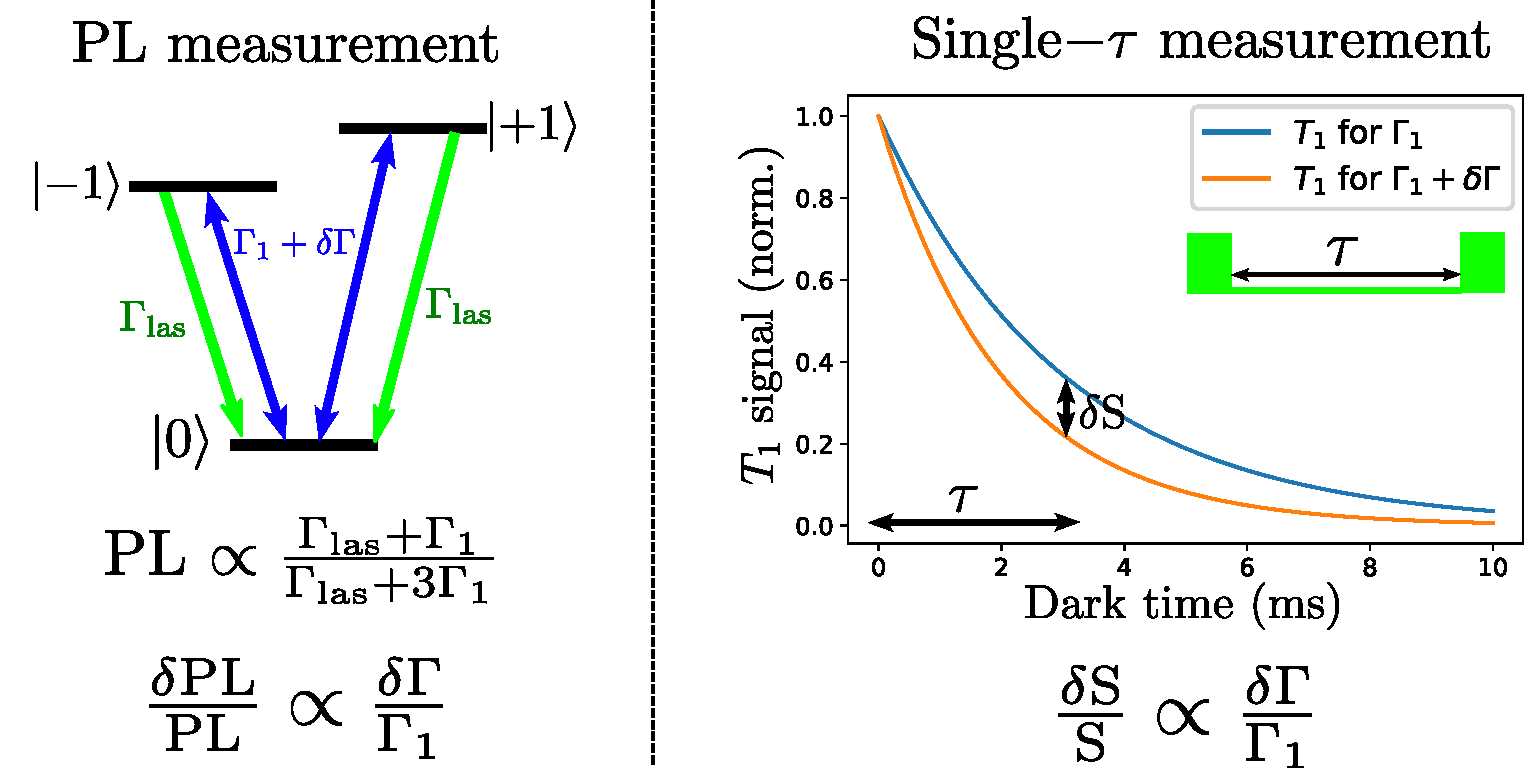
\includegraphics[width=0.9\textwidth]{Figures/relaxo_pulsed_continuous}
\caption{Representation of the two relaxometry protocol. Left : representation of the three level system of the NV center with the polarization rate $\Gamma_{\rm las}$ and spin decay rates $\Gamma_1=1/T_1$ and the perturbation $\delta \Gamma$. Right: simulation of a $T_1$ measurement for $1/\Gamma_1=3\ \rm ms$ and $1/(\Gamma_1+\delta \Gamma)=2\ \rm ms$. $\delta \rm S$ represents the maximum difference in signal between the two curves for a dark time $\tau$.}
\label{T1 vs PL}
\end{figure}

There are two ways to measure a change in the spin $T_1$, as represented on Fig. \ref{T1 vs PL}. The first and most basic method simply consist in monitoring the PL of the NV centers : since the PL is proportional to the population in the $\ket{0}$ state, which itself results from an equilibrium between the polarization rate $\Gamma_{\rm las}$ and the spin decay rate $\Gamma_1=1/T_1$. A change in $\Gamma_1$ will therefore conduct to a new equilibrium with a different PL. For a small enough change $\delta \Gamma << \Gamma_1$, we can consider that we remain in the linear regime, hence why $\frac{\delta \rm PL}{\rm PL} \propto \frac{\delta \Gamma}{\Gamma_1}$.

The second method is a pulsed sequence referred as single$-\tau$ measurement, used for example in \citep{pelliccione2014two, schmid2015relaxometry, tetienne2016scanning}. It simply consists in a $T_1$ measurement sequence (as seen in chapter 1) where you first polarize the spins in the $\ket{0}$ state with a laser pulse and read out the spin state with a second laser pulse after a dark time $\tau$. In this case however, instead of scanning the time $\tau$, you fix its value to maximize the sensitivity in a change of $T_1$ (typically $\tau \approx T_1$). Again, assuming you are in the linear regime, you observe a change in signal proportional to the change in $\Gamma_1$ : $\frac{\delta \rm S}{\rm S} \propto \frac{\delta \Gamma}{\Gamma_1}$.

It is argued in \citep{finco2021imaging} that both methods result in similar signal to noise ratio: in the first case you need to adjust $\Gamma_{\rm las} \sim \Gamma_1$ to maximize the PL contrast, meaning that the laser power used is very far from the saturation limit (typically $\Gamma_1 \approx 10^3\ \rm s^{-1}$ and $\Gamma_{\rm sat} = 5\cdot10^6\ \rm s^{-1}$\citep{dreau2011avoiding}), while the second method needs to wait a time $\tau \sim T_1$ between each measurement, which result in a similar PL count and shot noise limit in both case.

On a technical level, the PL-based method is easier to implement since it does not require the use of a pulsed laser, and uses an overall smaller laser power, however it is more sensitive to drifts and changes in the optical setup. Most of the relaxometry measurement in this manuscript were performed using a PL-based detection.

\subsection{Comparison with DEER protocol}

\begin{figure}[h]
\centering
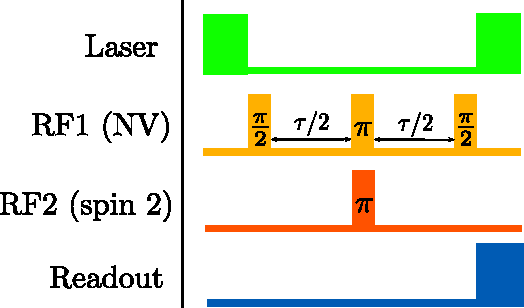
\includegraphics[width=0.5\textwidth]{Figures/DEER}
\caption{Pulse sequence of the DEER protocol}
\label{DEER}
\end{figure}

Outside of cross-relaxations, another protocol exists to address dark spin resonance with NV centers, based on a modification of the NV $T_2$ time \citep{serbyn2014interferometric}. This protocol called double electron-electron resonance (DEER) is depicted on Fig. \ref{DEER}. The pulse sequence consist in a spin-echo sequence on the NV center, as described in chapter 1, with a simultaneous $\pi-$pulse on the probed dark spins during the rephasing pulse on the NV centers. This additional pulse means that the static (or slowly variable) contribution of the probed spins to the $T_2^*$ of the NV center wont be rephased. The newly measured $T_2$ time should therefore be slightly shorter:

\begin{equation}
\frac{1}{T_2^{\rm DEER}}=\frac{1}{T_2^{\rm echo}} + \delta \Gamma,
\end{equation}

where $\delta \Gamma$ is the contribution of the dark spin to the $T_2^*$ of the NV center through NV-dark spin dipole-dipole interaction.

By scanning the frequency of the second microwave (RF2) and monitoring the $T_2$ time of the NV centers, one can therefore find dark spin resonance without having to bring them to resonance with NV centers, which can be useful when the dark spin resonance is very far detuned from the NV one.

While both cross-relaxation and DEER measure the dipole-dipole coupling of dark spins to an NV center, there are several differences between the two protocols :

Frist, the two protocols do not measure the same elements of the dipole-dipole Hamiltonian: CR measures the off-diagonal elements $\Omega_{\rm CR}=\mel{i,j}{\mathcal{H}_{\rm dd}}{j,i}/\hbar$ which are responsible for the flip-flops or double flips, while DEER measures the diagonal elements $\Omega_{\rm DEER}=\mel{i,j}{\mathcal{H}_{\rm dd}}{i,j}/\hbar$ which are responsible for the pure dephasing. These terms however are on average of the same amplitude, and when averaging over an ensemble we can consider $\Omega_{\rm CR} \sim \Omega_{\rm DEER}$

Second and more importantly, the scaling is not the same in both cases : CR measures a change in the NV decay rate $\Gamma_1=1/T_1$ which is proportional to $\Omega_{\rm CR}^2$, as given by eq. \ref{delta gamma 1}, while DEER measures a change in $\Gamma_2=1/T_2$ which is proportional to $\Omega_{\rm DEER}$, as given by eq. \ref{Gamma2 P1}. This means that the signal of CR scales quadratically with the impurity concentration, while the DEER signal scales linearly with it. CR is therefore more suited to probe concentrated impurities, when the average distance between the NV and the probed spin is small.

\section{Choice of the $\mathbf{B}$ scan orientation}

Since relaxometry does not rely on a microwave field, the only parameter left to tune is the external magnetic field, which is often scanned with an electromagnet. Due to the strong NV anisotropy however, the direction along which $\mathbf{B}$ is scanned plays a crucial role in the ability to detect dark spins.


\section{Attribution of the VH$^-$ and War1 lines}


\printbibliography
\end{document}